\documentclass[11pt]{article}
\usepackage[margin=1in]{geometry}
\usepackage{graphicx,amsmath,booktabs,hyperref,natbib}
\title{How much of the GLM-HMM's hidden-state structure in mouse decision-making is observable history? A decomposition with simulation-based calibration}
\author{Anas Nadeem\\ \small Independent researcher, Hong Kong \\ \small \texttt{anasnadeem30@gmail.com}}
\date{Preprint draft}
\begin{document}
\maketitle

\begin{abstract}
Generalized linear model--hidden Markov models (GLM-HMMs) are widely used to describe mouse perceptual decision-making as switches between a small number of persistent strategies. They are usually compared against simple baselines (a lapse model, a plain GLM, a slowly drifting GLM), not against stateless models that already use rich choice and outcome history. We ask how much of the GLM-HMM's held-out advantage survives such baselines, using 33 mice from nine laboratories in the public International Brain Laboratory (IBL) dataset (1.15 million block-task trials). A stateless logistic model with exponentially weighted action, stimulus and accuracy histories and within-session time recovers a median 83\% (IQR 72--92\%) of the held-out log-likelihood gain of a 3-state GLM-HMM over a four-input GLM. A GLM-HMM fit with the same covariates still wins in 33/33 mice, but an i.i.d.\ mixture of GLMs that has no Markov persistence reaches a median 92\% (IQR 85--97\%) of that remaining gain; temporal persistence adds only about $+0.005$ bits/trial. Closed-loop simulations calibrate the comparison: no persistence is detected in data generated by a stateless model or by an i.i.d.\ mixture, a persistent HMM yields $+0.024$ bits/trial, and with only the standard four inputs the GLM-HMM shows apparent persistence even on purely stateless data ($+0.076$ bits/trial). Much of the state structure attributed to GLM-HMMs in this task is therefore recoverable from observable history and trial-to-trial mixing of response policies, and comparisons made with few inputs overstate the evidence for persistent states. We release code and a calibration protocol that can be applied to other GLM-HMM datasets.
\end{abstract}

\section{Introduction}
Animals performing the same task do not behave the same way from trial to trial. \citet{ashwood2022} showed that a GLM-HMM, in which each hidden state has its own logistic regression from task variables to choice, describes IBL mouse choices better than a lapse model, a plain GLM and a continuously drifting GLM (PsyTrack; \citealt{roy2021}). The fitted states, an engaged state and states biased toward one side, last tens of trials. Later work has used GLM-HMMs on IBL data to study what drives switches between states \citep{mohammadi2025} and related models, such as an infinite semi-Markov HMM, to study learning \citep{bruijns2025}.

Two facts motivate a closer look at the baselines. First, the stateless models used for comparison in the original analysis did not include rich history terms. Second, \citet{findling2025} found that, on the IBL block task, the best stateless description of the animals' prior is an action kernel: an exponentially weighted average of recent choices (median decay about 5 trials), better than the Bayes-optimal prior. A GLM-HMM biased state may be, in part, such a kernel expressed through discrete states. We are not aware of work that asks how much of the GLM-HMM gain a strong stateless history model removes, nor whether the remaining gain requires temporal persistence rather than trial-by-trial mixing of response policies. This paper does both and calibrates the answer by simulation.

\paragraph{Contributions.} (i) A decomposition of the GLM-HMM's held-out gain into stateless history, non-persistent mixing, and persistence, for 33 IBL mice. (ii) A persistence control: a mixture of GLMs fit by the same EM procedure but with every row of the transition matrix equal to the marginal state distribution. (iii) A closed-loop simulation calibration showing when the persistence test does and does not return false positives, including a warning that few-input GLM-HMMs show apparent persistence in stateless data.

\section{Methods}
\paragraph{Data.} Public IBL behavioural data \citep{ibl2021}: 33 mice from nine laboratories, 1{,}149{,}100 trials after dropping no-go trials, using trials after the first 90 of each session (20/80 stimulus blocks). Choice is binary (right vs.\ left). This is a different trial subset from the first-90-trial, 50/50 segment analysed by \citet{ashwood2022}, so our baseline GLM and GLM-HMM numbers are not directly comparable to theirs.

\paragraph{Models.} All models are Bernoulli GLMs, $P(y_t=1)=\sigma(w\cdot x_t)$. The four-input set X0 is signed stimulus, previous choice, win-stay-lose-shift and bias. S1 adds five action kernels (exponentially weighted averages of past choices, $\tau\in\{2,5,10,20,40\}$ trials). S2 adds stimulus kernels ($\tau=5,20$), accuracy EWMAs ($\tau=5,20$, centred), two stimulus$\times$accuracy terms and the fraction of the session elapsed. All history features use strictly past trials within a session. The GLM-HMM has $K$ hidden states with state-specific weights, Markov transitions, and EM fitting (own implementation, forward--backward, weighted logistic M-step, best of three initialisations by training likelihood). The i.i.d.\ mixture (MIX) is the same model with $A_{ij}=\pi_j$ for all $i$. Comparing a hidden Markov model with a mixture that has the same emissions but no temporal structure has precedent in resting-state fMRI \citep{ezaki2021}; here the emissions are behavioural GLMs, the comparison is in held-out bits per trial, and it is calibrated in closed loop.

\paragraph{Evaluation.} For each mouse, 5-fold cross-validation with folds grouped by session; the score is held-out log-likelihood per trial in bits, summed over folds. Reported fractions are per-mouse ratios; summaries are medians with interquartile ranges unless stated.

\paragraph{Calibration.} For each mouse we replay the real stimulus sequence and true correct side in closed loop and generate choices from (a) the fitted stateless S2 GLM, (b) a fitted 3-state GLM-HMM on X0, or (c) a fitted i.i.d.\ mixture on X0, so that history features evolve from the simulated choices. The same cross-validated pipeline is then run on the simulated data (one replicate per mouse and generator).

\section{Results}
\paragraph{Stateless history recovers most of the GLM-HMM gain.} Over the four-input GLM, the 3-state GLM-HMM (X0) improves held-out likelihood by 0.113 bits/trial, in 33/33 mice (Fig.~\ref{fig:dec}A). Adding action kernels alone (S1) recovers a median 64\% of this, and the full stateless set S2 a median 83\% (IQR 72--92\%). The GLM-HMM with X0 inputs still beats the S2 GLM in 32/33 mice, but the median margin is only 0.016 bits/trial.

\paragraph{The remaining gain is mostly non-persistent.} With S2 inputs the GLM-HMM beats the S2 GLM in 33/33 mice (mean $+0.059$ bits/trial). An i.i.d.\ mixture with the same inputs captures a median 92\% (IQR 85--97\%) of that gain (mean MIX3(S2) $-0.4965$ vs.\ HMM3(S2) $-0.4914$ bits/trial). The HMM's advantage over the mixture is small, $+0.005$ bits/trial (median $+0.004$), though consistent (30/33 mice, Wilcoxon signed-rank $p=10^{-7}$). With the four standard inputs the same comparison gives $+0.043$ bits/trial (33/33): persistence appears more important when history is not modelled.

\paragraph{Calibration.} Fig.~\ref{fig:cal} and Table~\ref{tab:cal} show the same comparison on simulated data. With S2 inputs the HMM--mixture difference is $-0.0003$ bits/trial for stateless data and $-0.001$ for i.i.d.-mixture data (HMM ahead in 4/33 mice), whereas persistent-HMM data give $+0.024$ (33/33). Real mice ($+0.005$) lie much nearer the no-persistence end. With only four inputs, stateless data produce an HMM--mixture difference of $+0.076$ bits/trial, larger than the real-mouse value of $+0.043$: unmodelled history can be absorbed by persistent hidden states.

\begin{table}[h]\centering\small
\begin{tabular}{lrrr}\toprule
Data from & HMM$-$MIX (X0) & HMM$-$MIX (S2) & MIX share of HMM gain (S2)\\\midrule
Stateless S2 GLM & $+0.076$ & $-0.0003$ & --\\
i.i.d.\ mixture & $-0.0006$ & $-0.001$ & 101\%\\
Persistent HMM & $+0.064$ & $+0.024$ & 62\%\\
Real mice & $+0.043$ & $+0.005$ & 92\%\\\bottomrule
\end{tabular}
\caption{Calibration of the persistence test (bits/trial, medians over 33 mice; one simulated replicate per mouse).}\label{tab:cal}
\end{table}

\begin{figure}[h]\centering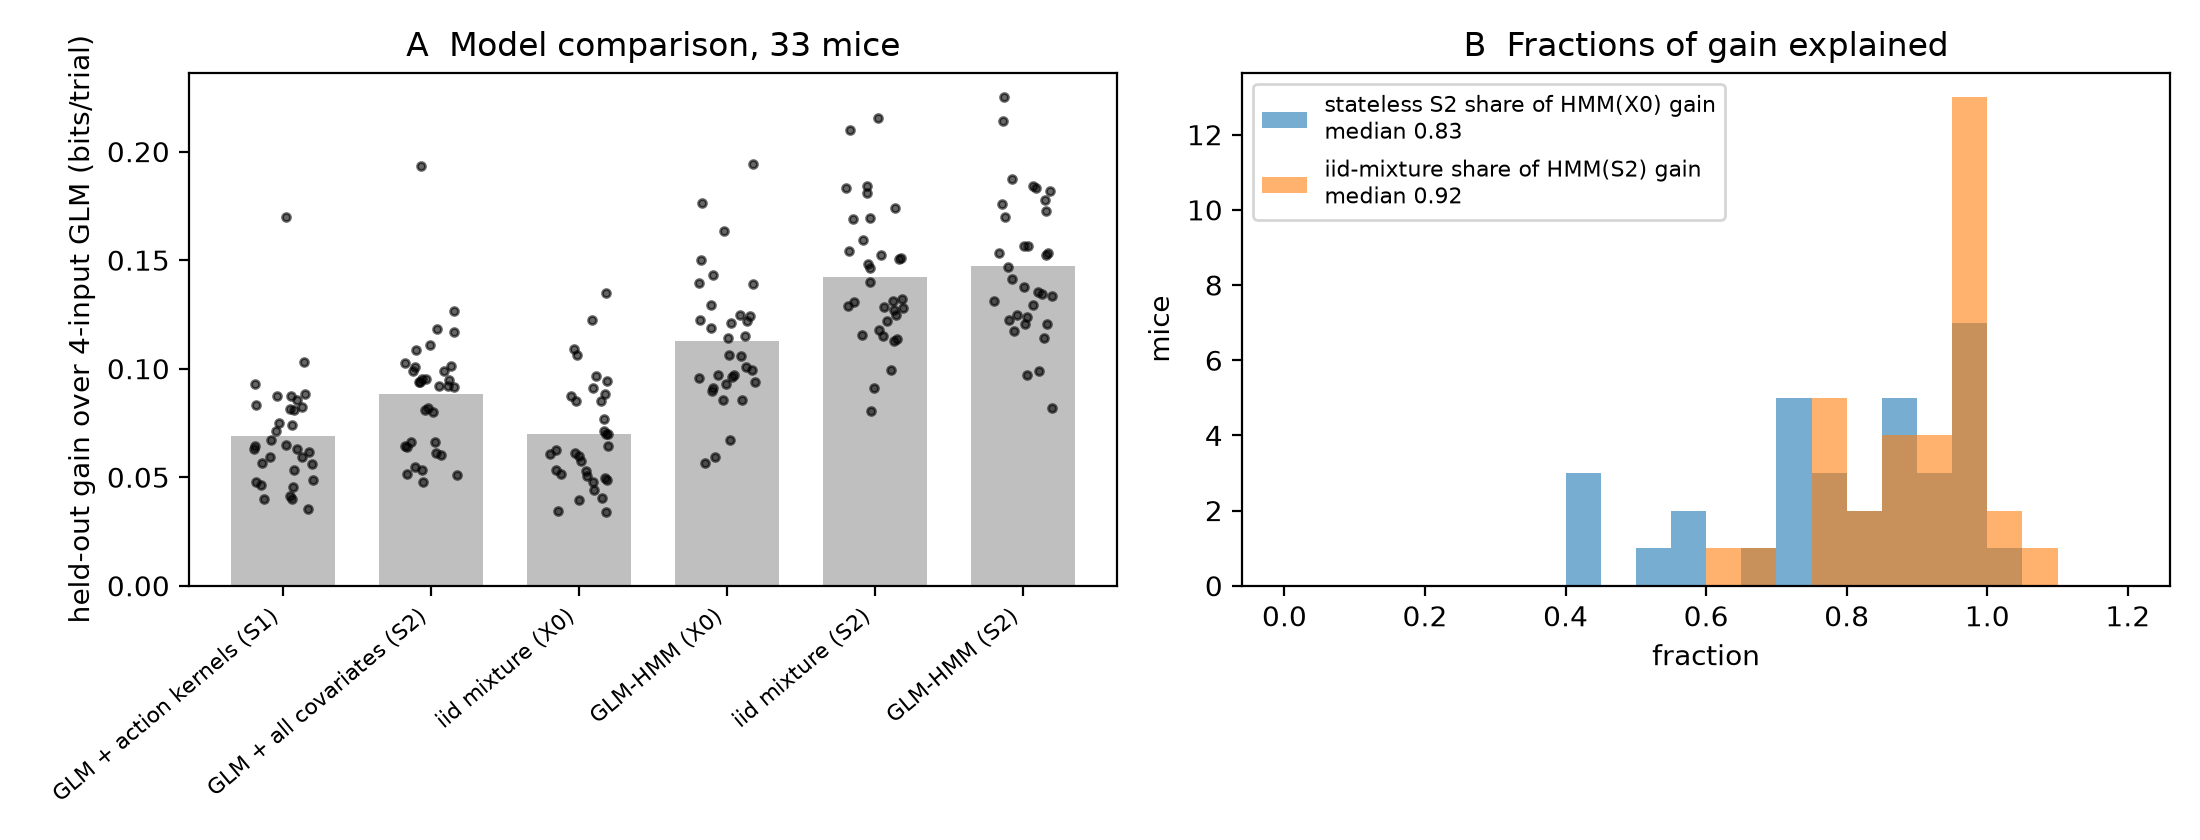
\includegraphics[width=\textwidth]{fig1_decomposition.png}
\caption{Decomposition of held-out gain over the four-input GLM. (A) Gain by model, dots are mice. (B) Fraction of the HMM gain explained by stateless S2 (relative to HMM on X0) and by an i.i.d.\ mixture (relative to HMM on S2).}\label{fig:dec}\end{figure}
\begin{figure}[h]\centering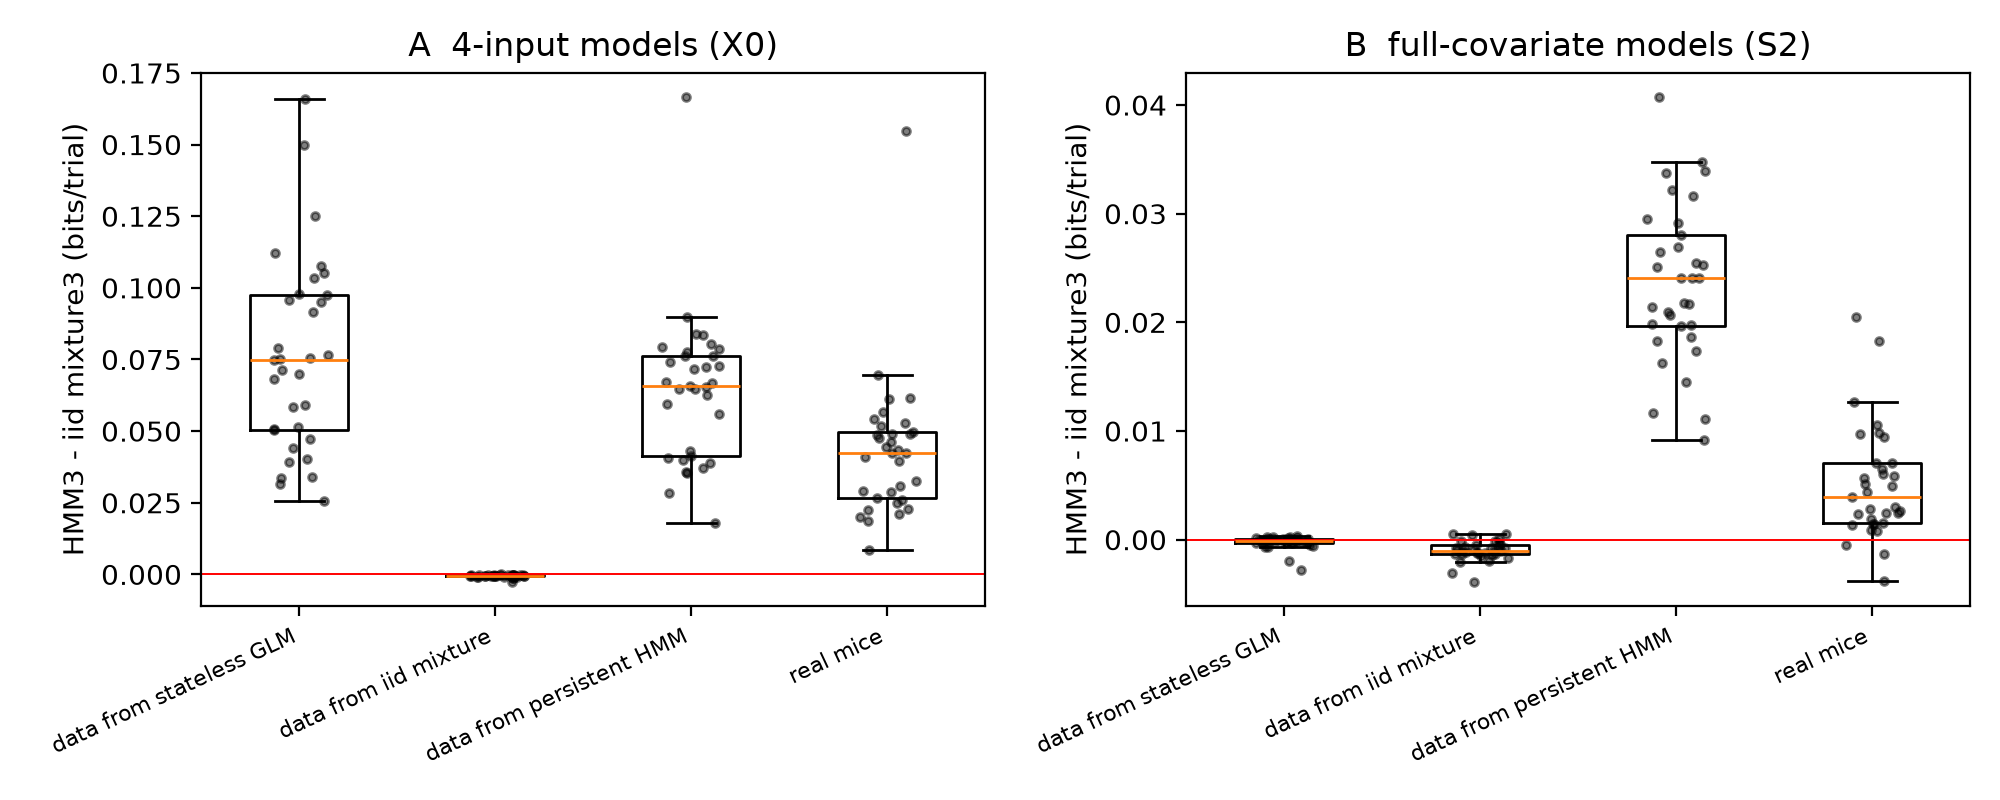
\includegraphics[width=\textwidth]{fig2_calibration.png}
\caption{HMM minus i.i.d.\ mixture held-out likelihood on simulated and real data. (A) Four-input models. (B) Full-covariate models. Persistent-HMM data produce a clear gap with full covariates; real mice sit close to the no-persistence cases.}\label{fig:cal}\end{figure}

\paragraph{Number of states.} With S2 inputs, the HMM--mixture gap grows slowly with the number of states: $+0.0026$, $+0.0051$, $+0.0067$ and $+0.0071$ bits/trial for $K=2,3,4,5$ (HMM ahead in 29, 30, 31 and 31 of 33 mice), and the mixture's share of the HMM gain over the S2 GLM falls from 96\% to 92\%, 90\% and 89\% (medians). All remain far below the $+0.024$ bits/trial obtained from simulated persistent-HMM data at $K=3$. We did not explore $K>5$.

\section{Discussion}
In this cohort, a GLM-HMM's apparent states are largely explained by observable history plus trial-to-trial mixing of response policies. We do not claim that mice lack internal states. Persistence adds a small, consistent amount, and our stateless features may be proxies for slow internal variables (the S2 accuracy and time terms, in particular, are cheap readouts of engagement). The result instead says that a hidden-state interpretation requires comparison against strong history baselines and a persistence control, and that few-input GLM-HMM comparisons can mistake unmodelled history for persistence.

\paragraph{Relation to prior work.} Our stateless S2 model extends the action-kernel account of \citet{findling2025} as a comparator for the GLM-HMM. \citet{mohammadi2025} found that past choices and stimuli predict state switches, which is compatible with a large history component. The infinite semi-Markov HMM of \citet{bruijns2025} models dwell times during learning; our question concerns steady-state behaviour and whether persistence is needed at all. The i.i.d.\ mixture still has several latent response policies, so our result supports ``multiple policies without Markov persistence'' and not ``no discrete strategies''. \citet{carandini2024} argues that choices are well described by logistic combinations of inputs, past actions and value without hidden states, and \citet{bruijns2025b} fit flexible models to 139 IBL mice and report continual fluctuations in engagement; \citet{nicoletti2026} report that GLM-HMMs, including history-dependent variants, fail to capture mouse behaviour in a reversal task. None of these quantifies the GLM-HMM gain left after strong stateless baselines or tests persistence directly (\citealt{urai2025} reviews related HMM and autoregressive approaches). A continuously drifting-weights model (PsyTrack; \citealt{roy2021}) is another stateless alternative that we have not yet tested as a comparator.

\paragraph{Limitations.} One task and one dataset; block trials only; $K=3$ for the main analysis ($K\le5$ checked); hand-designed covariates (other stateless models could do better or worse); one simulated replicate per mouse and generators with X0-only emissions, so history-dependent hidden states are not covered; logistic EM convergence warnings in wide GLMs were not quantified; model comparison by held-out likelihood does not establish neural or causal state identity.

\paragraph{Code and data.} IBL data are public. Code and per-mouse results: \url{https://github.com/anasnadeem30/ibl-glmhmm-individuality} (folder \texttt{history\_baselines}).

\begin{thebibliography}{99}
\bibitem[Ashwood et~al.(2022)]{ashwood2022} Ashwood ZC, Roy NA, Stone IR, International Brain Laboratory, Urai AE, Churchland AK, Pouget A, Pillow JW. Mice alternate between discrete strategies during perceptual decision-making. \emph{Nat Neurosci} 25:201--212, 2022. doi:10.1038/s41593-021-01007-z.
\bibitem[Roy et~al.(2021)]{roy2021} Roy NA, Bak JH, Akrami A, Brody CD, Pillow JW. Extracting the dynamics of behavior in sensory decision-making experiments. \emph{Neuron} 109:597--610, 2021. doi:10.1016/j.neuron.2020.12.004.
\bibitem[Mohammadi et~al.(2025)]{mohammadi2025} Mohammadi Z, Ashwood ZC, International Brain Laboratory, Pillow JW. Identifying the factors governing internal state switches during nonstationary sensory decision-making. \emph{Nat Commun} 16:11684, 2025. doi:10.1038/s41467-025-66738-0.
\bibitem[Findling et~al.(2025)]{findling2025} Findling C, Hubert F, Acerbi L, et al.\ (International Brain Laboratory). Brain-wide representations of prior information in mouse decision-making. \emph{Nature} 645:192--200, 2025. doi:10.1038/s41586-025-09226-1.
\bibitem[Bruijns et~al.(2026)]{bruijns2025} Bruijns SA, International Brain Laboratory, Lau PYP, et al., Dayan P. Infinite hidden Markov models can dissect the complexities of learning. \emph{Nat Neurosci} 29:186--194, 2026 (online 2025). doi:10.1038/s41593-025-02130-x.
\bibitem[Bruijns et~al.(2025b)]{bruijns2025b} Bruijns SA, Eckstein MK, Dayan P. Low dimensional latent structure underlying the choices of mice. \emph{bioRxiv}, 2025. doi:10.1101/2025.08.08.669381.
\bibitem[Carandini(2024)]{carandini2024} Carandini M. Sensory choices as logistic classification. \emph{Neuron}, 2024. doi:10.1016/j.neuron.2024.06.016.
\bibitem[Nicoletti and Celani(2026)]{nicoletti2026} Nicoletti G, Celani A. Decoding behavior with minimal and interpretable agent models. \emph{PLoS Comput Biol}, 2026. doi:10.1371/journal.pcbi.1014585.
\bibitem[Urai(2025)]{urai2025} Urai AE. Structure uncovered: understanding temporal variability in perceptual decision-making. \emph{Trends Cogn Sci}, 2025. doi:10.1016/j.tics.2025.06.003.
\bibitem[Ezaki et~al.(2021)]{ezaki2021} Ezaki T, Himeno Y, Watanabe T, Masuda N. Modelling state-transition dynamics in resting-state brain signals by the hidden Markov and Gaussian mixture models. \emph{Eur J Neurosci} 54:5404--5416, 2021. doi:10.1111/ejn.15386.
\bibitem[IBL(2021)]{ibl2021} International Brain Laboratory, et al. Standardized and reproducible measurement of decision-making in mice. \emph{eLife} 10:e63711, 2021. doi:10.7554/eLife.63711.
\end{thebibliography}
\end{document}
